% !TEX root = ../../../under-spec-z.tex

\subsection{The Zariski topology} % (fold)
\label{sub:the_zariski_topology}

    \emph{Yet again, throughout this section we assume that $\smc$ is a cosmos and use $\dcat$ to refer to an arbitrary category.}

    \subsubsection{Zariski covers} % (fold)
    \label{ssub:zariski_covers}

        Our next goal is to define the \emph{Zariski topology on $\aff{\ccat}$}.
        Once again, we start by defining a certain type of morphism in $\aff{\ccat}$ and saying when a collection of such morphisms gives an \emph{open cover}.

        \begin{definition}[Zariski open {(Définition~2.9,~\S2.3,~p.15)}]\label{df:zariski-open-morphism}
            Let $f\colon A\to B$ in $\comm{\ccat}$.
            Then $f$ is
            \begin{enumerate}[(i)]
                \item \emph{flat} if the functor
                    \begin{equation*}
                        (\blank\otimes_A B)\colon\modc{A}\to\modc{B}
                    \end{equation*}
                    is exact\footnote{
                        We already know that this functor commutes with colimits, since $(\modc{A},\otimes_A,A)$ is closed (\cref{le:modc-a-cosmos-algc-a-bicomplete}), so it is exact if and only if it commutes with finite limits as well, i.e. if and only if it is left exact.
                    };
                \item an \emph{epimorphism} if, for all $X\in\comm{\ccat}$, the map
                    \begin{equation*}
                        (\blank\circ f)\colon\Hom(B,X)\to\Hom(A,X)
                    \end{equation*}
                    is injective;
                \item a \emph{finite presentation} if, for every filtered diagram\footnote{
                        That is, our diagram is \emph{non-empty} and such that
                        \begin{enumerate}[(i)]
                            \item for any two objects $x,y$ in the diagram there exists some object $k$ and arrows \mbox{$x\to k\leftarrow y$};
                            \item for any parallel arrows $f,g\colon x\to y$ there exists some object $k$ and an arrow $a\colon y\to k$ such that $af=ag$.
                        \end{enumerate}
                    } of objects
                    \begin{equation*}
                        \{X_i\in A/\comm{\ccat}\}_{i\in I},
                    \end{equation*}
                    the natural morphism
                    \begin{equation*}
                        \colim_i\Hom_{A/\comm{\ccat}}(B,X_i) \longrightarrow \Hom_{A/\comm{\ccat}}(B,\colim_i X_i)
                    \end{equation*}
                    is an isomorphism.
            \end{enumerate}
            We say that $f\colon\spec B\to\spec A$ in $\aff{\ccat}$ is \emph{Zariski open} (or an \emph{open Zariski immersion}) if the corresponding morphism $f\colon A\to B$ in $\comm{\ccat}$ is a flat epimorphism of finite presentation.
            % (where these three properties are as defined in \cref{tb:flat-epi-finite-presentation}).
        \end{definition}

        % \begin{table}[h!]
        %     \centering
        %     \begin{tabular}{llr}
        %         $f$ is \ldots & if \ldots & is \ldots\\
        %         \toprule
        %         a \emph{flat} morphism & $(\blank\otimes_A B)\colon\modc{A}\to\modc{B}$ & exact\\
        %         an \emph{epimorphism} & $(\blank\circ f)\colon\Hom(B,X)\to\Hom(A,X)$ & injective for all $X$\\
        %         of \emph{finite presentation} & $\spec$ & a
        %     \end{tabular}
        %     \caption{Possible properties of $f\colon A\to B$ in $\comm{\ccat}$}
        %     \label{tb:flat-epi-finite-presentation}
        % \end{table}

        \begin{definition}[fpqc and Zariski covers {(Définition~2.10,~\S2.3,~p.16)}]\label{df:fpqc-zariski-covers}
            A family of morphisms $\{\spec A_i\to\spec A\}_{i\in I}$ in $\aff{\ccat}$ is
            \begin{enumerate}[(i)]
                \item an \emph{fpqc cover} (or simply a \emph{flat cover}) if
                    \begin{enumerate}
                        \item for all $i\in I$, the morphism $\spec A_i\to\spec A$ is flat;
                        \item there exists some finite subset $J\subset I$ such that the functor
                            \begin{equation*}
                                \prod_{j\in J}(\blank\otimes_A A_j)\colon\modc{A}\to\prod_{j\in J}\left(\modc{A_j}\right)
                            \end{equation*}
                            is conservative\footnote{
                                By definition, this is just asking that $(\blank\otimes_A A_j)$ be conservative for each $j\in J$.
                            };
                    \end{enumerate}
                \item a \emph{Zariski cover} if
                    \begin{enumerate}
                        \item it is an fpqc cover;
                        \item for all $i\in I$, the morphism $\spec A_i\to \spec A$ is Zariski open.\qedhere
                    \end{enumerate}
            \end{enumerate}
        \end{definition}

        \emph{We are interested primarily in the Zariski topology, and the fpqc topology will be used essentially only for \elide(\cref{le:essential-image-is-fpqc})} (\S2.3~p.16~\P3).

        \bigskip

        Saying that a family of morphisms is a flat cover, in the sense of the above definition, is just another way\footnote{
            The only real difference between being a flat cover and being $M$-faithfully flat is that the former requires exactness of the change of base functor $(\blank\otimes_A A_i)$ whereas the latter requires only left exactness, but we know that this functor is right exact anyway, since it is left adjoint to the forgetful functor $\modc{A_i}\to\modc{A}$.
            Thus these two requirements coincide.
        } of saying it is $M$-faithfully flat, in the sense of \cref{ssub:fpqc_topology}.
        So we already know that flat covers give rise to a topology: the fpqc (or flat) topology.
        To show that the same is true for Zariski covers we need to show that the property of being Zariski open is preserved by pullbacks and is associative (in the sense of \cref{df:grothendieck-pretopology}), and also that isomorphisms are Zariski open.
        However, \cref{df:zariski-open-morphism} is phrased \emph{not} in terms of $\spec B\to\spec A$, but instead in terms of the corresponding \mbox{$A\to B$}.
        So we need to check that these properties of morphisms of \emph{commutative monoids} are stable under \emph{pushouts}.
        Stability of finite presentation follows from a lengthy definition chase, and epimorphisms are always stable under pushouts\footnote{
             \cite[Proposition~2.5.3(1)]{Borceux:1994ws}
        }.
        As for flatness, the fpqc topology already tells us that flatness is preserved.

        \begin{definition}[Zariski topology]
            The topology on $\aff{\ccat}$ generated\footnote{
                As in \cref{le:m-t-grothendieck-pretopology}.
            } by Zariski covers is called the \emph{Zariski topology}.
        \end{definition}

        \begin{note}
            Because we require both fpqc and Zariski covers to be finitely conservative, a sieve $S$ on $\spec A$ is in the generated topology if and only if it contains some cover if and only if it contains the finite conservative subset of that cover.
            This means that these pretopologies are \emph{quasi-compact}, i.e. generated by finite covering families.
            For more, see the beginning of \cite[\S~IX.11]{MacLane:1992uz}.
        \end{note}
        
    % subsubsection zariski_covers (end)


    \subsubsection{Sheaves} % (fold)
    \label{ssub:sheaves}

        Just as in classical algebraic geometry, now that we have some topology we can introduce the idea of `gluing together' affine schemes to obtain \emph{schemes}.
        Fundamental to this idea is the definition of a \emph{sheaf}.

        \begin{definition}[Sheaves on a site]\label{df:sheaves-on-site}
            Let $(\dcat,J)$ be a site\footnote{
                \cref{df:site}
            } and $F\in\PShv(\dcat)$ some presheaf\footnote{
                \cref{df:presheaves}
            }.
            We say that $F$ is a \emph{$J$-sheaf} (or simply a \emph{sheaf} if the context is clear) if, for all objects $X\in\dcat$ and covering sieves $S\in J(X)$ on $X$, the natural map
            \begin{equation*}
                \Hom(\Hom(\blank, X), F)\longrightarrow\Hom(S,F)
            \end{equation*}
            induced by the inclusion $S\hookrightarrow\Hom(\blank, X)$ is a bijection.

            We write $\Shv^J(\dcat)$ to be the category of sheaves on $(\dcat,J)$, a full subcategory of $\PShv(\dcat)$.
        \end{definition}

        If we have a pretopology then we can rewrite this definition in a way which is sometimes easier to apply in practice, and also gives a better geometric intuition.

        \begin{lemma}[Sheaves on a presite]\label{le:sheaves-on-presite}
            Let $(\dcat, C)$ be a presite\footnote{
                This is not standard terminology, but we define a \emph{presite} as a pair $(\dcat,C)$ consisting of a category $\dcat$ and a Grothendieck pretopology $C$ on $\dcat$.
                Given such a pair, we can talk about the \emph{site that it generates} by endowing $\dcat$ with the Grothendieck topology generated by $C$.
            }, $(\dcat, J)$ the site that it generates, and $F\in\PShv(\dcat)$.
            Then $F\in\Shv^{J}(\dcat)$ if and only if, for all objects $X\in\dcat$ and covering families $\{X_i\to X\}_{i\in I}\in C(X)$ of $X$,
            \begin{equation*}
                F(X) = \eq\left( \prod_{i\in I}F(X_i)\rightrightarrows\prod_{j,k\in I}F(X_j\times_X X_k) \right)
            \end{equation*}
            (where the \emph{equaliser} $\eq$ is the dual notion to the coequaliser\footnote{
                \cref{df:coequaliser}
            }).
        \end{lemma}

        \begin{proof}
            \cite[\S III.4,~Proposition 1]{MacLane:1992uz}
        \end{proof}

        As for how this provides us with some intuition, let us return to the example of $\Op{T}$.
        In this category, pullbacks correspond to intersection, and we think of presheaves as being functions on the open sets that take inclusion maps to restriction maps.
        \cref{le:sheaves-on-presite} says that $F$ is a sheaf if and only if, when we piece together all of the $F(X_i)$ that agree on overlaps (this is the equaliser term), we get exactly $F(X)$, for any cover ${X_i}$ of $X$.
        This is just the (classical) presheaf condition -- see \cref{fg:sheaves}.
        % Then the equaliser condition in \cref{le:sheaves-on-presite} says that a presheaf $F$ is a sheaf if and only if, for all open sets $X$ and all Zariski open covers\footnote{
            % Here we would need to unpack some definitions: this doesn't have to hold for \emph{any} open cover $\{X_i\}$ of $X$; it only has to hold for Zariski covers (\cref{df:fpqc-zariski-covers}).
        % } $\{X_i\}$ of $X$,
        % \begin{equation*}
            % \left(F\big|_{X_i}\right)\bigg|_{X_i\cap X_j} = \left(F\big|_{X_j}\right)\bigg|_{X_i\cap X_j}
        % \end{equation*}
        % which coincides with our classical intuition of what a sheaf should be.

        \begin{figure}[h]
            \centering
            \frame{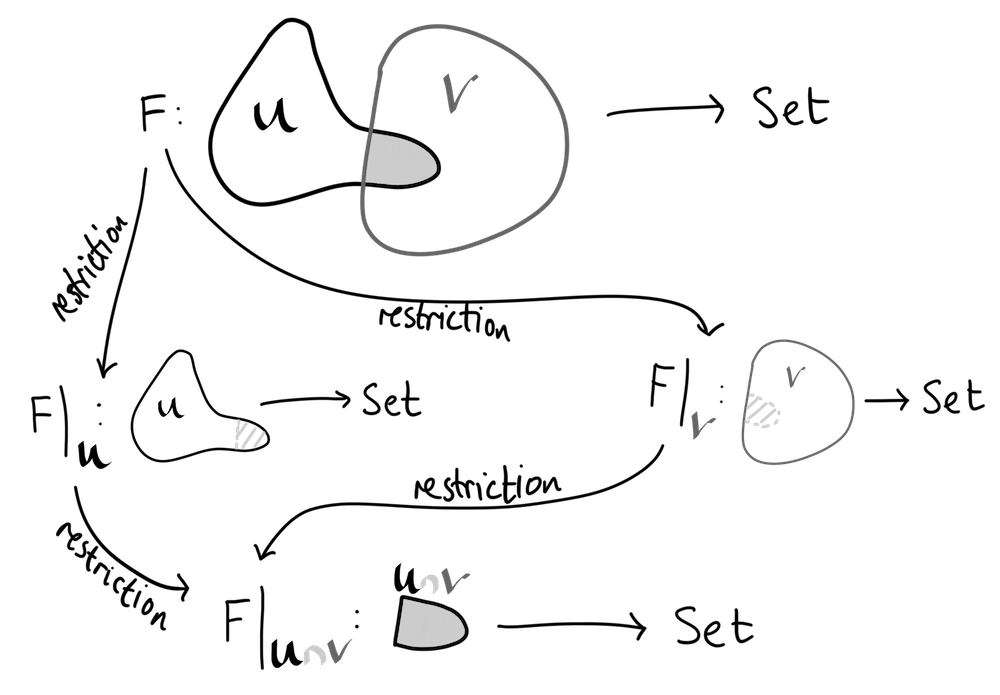
\includegraphics[width=.85\textwidth]{images/sheaves.png}}
            \caption{The fact that we always have a morphism from $F(X)$ to the equaliser in \cref{le:sheaves-on-presite} corresponds to the classical presheaf condition: for presheaves on a topological space it doesn't matter whether we restrict $U\cup V$ to $U\cap V$ via $U$ or via $V$}
            \label{fg:sheaves}
        \end{figure}

        \bigskip

        Since the Zariski topology is coarser (see \cref{fg:zariski-vs-fpqc-topology}) than the fpqc topology, the collection of fpqc covering sieves on some object is at least as large as the collection of Zariski covering sieves.
        This means that asking for the map induced by inclusion in \cref{df:sheaves-on-site} to be a bijection for all covering sieves on an object is a stricter condition in the fpqc topology than in the Zariski topology.
        So being an fpqc sheaf implies being a Zariski sheaf, but the converse doesn't necessarily hold.
        Thus we have the subcategories
        \begin{equation*}
            \Shv^{\text{fpqc}}(\aff{\ccat})\subset\Shv^{\text{Zar}}(\aff{\ccat})\subset\PShv(\aff{\ccat}).
        \end{equation*}

        \begin{note}
            As already stated, our primary interest is the Zariski topology, so whenever we speak of sheaves without reference to a specific topology it is assumed that we mean Zariski sheaves.
            Similarly, we write $\Shv(\aff{\ccat})=\Shv^{\text{Zar}}(\aff{\ccat})$.
        \end{note}

        \begin{figure}[h]
            \centering
            \frame{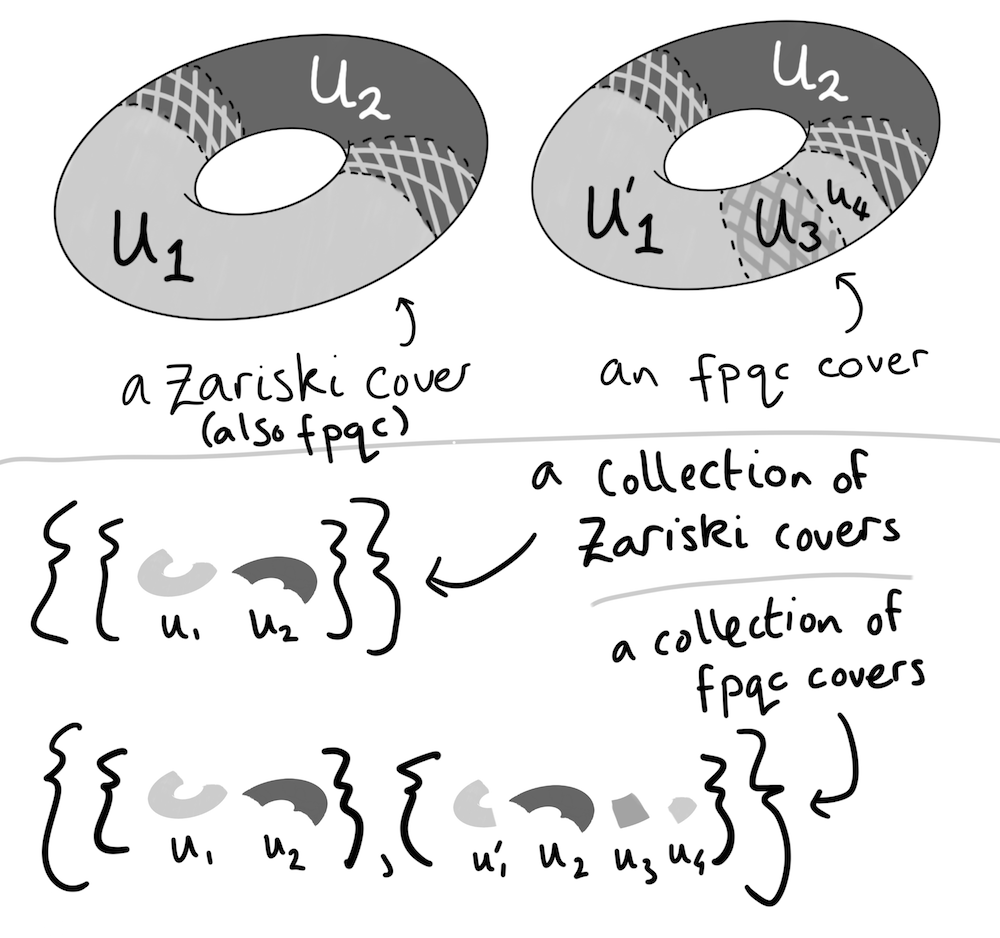
\includegraphics[width=.8\textwidth]{images/zariski-vs-fpqc-topologyNEW.png}}
            % \caption{Two topologies $\sigma,\tau$; here $\tau$ is coarser than $\sigma$}
            \caption{The Zariski topology is \emph{coarser} than the fpqc topology, i.e. it has fewer open sets, so every Zariski cover is also an fpqc cover -- the sheaf condition `reverses' this inclusion: there are \emph{more} fpqc covers than Zariski, hence \emph{fewer} fpqc sheaves than Zariski (and \textbf{maybe} hence \emph{more} fpqc schemes (something we don't define) than Zariski; see \cref{fg:hierarchy} for a similar conjecture)}\label{fg:zariski-vs-fpqc-topology}
        \end{figure}

        In \cref{ssub:motivating_example} we identified $\aff{k}$ with its essential image in $\PShv(\aff{k})$ under the Yoneda embedding, and we can do the same here: identify $\aff{\ccat}$ with its essential image in $\PShv(\aff{\ccat})$ under the Yoneda embedding.
        It turns out, however, that we can actually come up with a stronger result.

        \begin{lemma}[\mbox{}{(Corollaire~2.11,~\S2.3,~p.17)}]\label{le:essential-image-is-fpqc}
            For all $X\in\aff{\ccat}$ the presheaf $Y_X$ coming from the Yoneda embedding\footnote{
                \cref{le:yoneda-lemma,le:yoneda-embedding}
            } is an fpqc sheaf.
        \end{lemma}

        \begin{proof}
            The proof in \cite{Toen:2005wxa} uses stacks; see \cref{nt:no-theorem-2.5}.
        \end{proof}

        Firstly, this exactly says that the fpqc topology (and thus the Zariski topology, since it is coarser) is \emph{subcanonical}: all representable presheaves are fpqc sheaves.
        Secondly, this means we have the equivalence of categories
        \begin{equation}\label{eq:both-types-of-affine-schemes}
            \aff{\ccat}\equiv\ASch(\ccat) 
        \end{equation}
        where we define the full subcategory $\ASch(\ccat)\subset\Shv(\aff{\ccat})$ by
        \begin{equation*}
            \ASch(\ccat)=\{X\in\Shv(\aff{\ccat}) \mid X\cong \Hom_{\aff{\ccat}}(\blank,\spec A)\text{ for some } \spec A\in\aff{\ccat}\}.
        \end{equation*}
        We call the objects of $\ASch(\ccat)$ \emph{affine schemes}.
        
        \begin{definition}[Affine schemes over $\ccat$]\label{df:affine-schemes-general}
            From now on we use the phrase `affine scheme' interchangeably, to mean an object of either $\aff{\ccat}$ or $\ASch(\ccat)$.
            We often use the same notation for both as well (so for $\spec A\in\aff{\ccat}$ we also write $\spec A\in\ASch(\ccat)$ to mean $Y_A=\Hom(\blank,\spec A)$, and vice versa).
        \end{definition}
        
    % subsubsection sheaves (end)

% subsection the_zariski_topology (end)








    \clearpage
